\section{Grundlagen}\label{kap:grund}
In diesem Kapitel wird zunächst erörtert was genau eine Speicherprogrammierbare Steuerung eigentlich ist und wo sie eingesetzt wird und wieso man sie eigentlich benötigt. Des weiteren wird am Beispiel einer Easy Kleinsteuerung beschrieben, wie hier die Erstellung eines Logikprogramms von statten geht. Im weiteren Verlauf wird ein Logikprogramm vorgestellt und erklärt in welche logischen Teile die Funktion aufgeteilt wird. Zuletzt bietet dieses Kapitel auch Einblick in die Rahmenbedingungen der Arbeit wie die Versionsverwaltung, die Entwicklungsumgebung sowie eingesetzte Softwarebibliotheken. 
%\subsubsection{Motivation}
\subsection{Prinzip Speicherprogrammierbare-Steuerung}
Die Grundsätzliche Funktion einer Speicherprogrammierbaren Steuerung oder \texttt{SPS} ist, die Ermittlung der Ausgangswerte bzw. Schalterstellung durch eine logische Verknüpfung der Eingangswerte.\cite{BOOK:SPS} Wie in Beispiel der \autoref{fig:plcFigure} zu sehen, könnte ein an einen Eingang angeschlossener Schalter als Sensor dienen. Als Aktor könnte eine Leuchte dienen. Der Benutzer der Steuerung muss nun durch eine Logik für jeden Ausgang festlegen, in welchen Fällen dieser Ausgang aktiv sein soll. Doch wieso schließt man dann nicht einfach die Leuchte direkt an den Schalter an? Dies wäre bei einer einfachen Lampensteuerung sicherlich zu bevorzugen, jedoch handelt es sich bei den Szenarien die mit einer solchen Steuerung realisiert werden für Gewöhnlich um deutlich komplexere Verschaltungen. Bei der klassischen Installation für eine Torsteuerung Beispielsweise, wären mehrere Elektromechanische Relais, auch Schütze genannt nötig. Zudem bedürfte ein automatisches schließen des Tores ein Zeitrelais. Der Verdahtungsaufwand und Platzbedarf wären relativ hoch. Führt man stattdessen jedoch alle benötigten Sensoren auf eine Speicherprogrammierbare Steuerung wird der Verdrahtungsaufwand erheblich reduziert, was zu einer höheren Übersichtlichkeit führt und weniger Potential für Fehler bietet. Auch zieht eine Änderung im Logischen verhalten der Steuerung dann für gewöhnlich keinerlei Verdrahtungsänderungen mehr nach sich. Zuletzt sind auch die Kosten für Speicherprogrammierbare Steuerungen inzwischen auf einem Niveau, was klassische Steuerungen schnell unwirtschaftlich macht. 
\newcommand*{\quelle}{% 
	\footnotesize Quelle: 
} 

\begin{figure}[H]
	\centering
	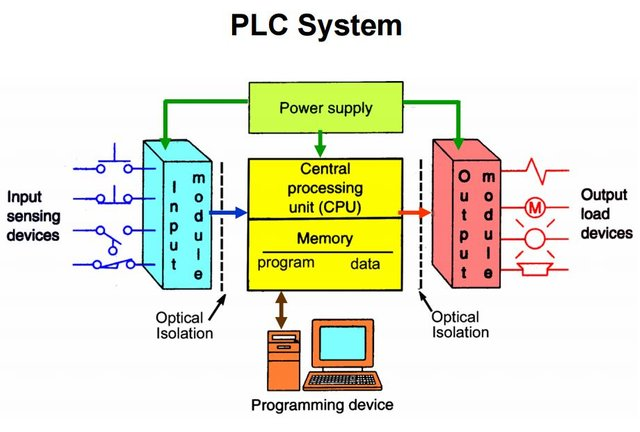
\includegraphics[ clip, trim=0.5cm 0.5cm 0.5cm 0.5cm, width=0.70\textwidth]{./images/plc.JPG}	\caption[Blockdiagramm SPS]{Blockdiagramm SPS \cite{URL:PLC}}
	\label{fig:plcFigure}
\end{figure}

%\subsection{Konzept?}
\subsection{Ausgangssituation} 

Als Vorbild für dieses Projekt dient die Kleinsteuerung Easy vom Hersteller Eaton. Das Einstiegsmodell bietet hier acht Eingänge und vier Ausgänge. Das Logikprogramm, welches die Eingänge der Steuerung logisch mit den Ausgängen verbindet wird hier, auf einem kleinen Display, direkt am Gerät erstellt. Dabei stehen neben den physikalischen Ein- und Ausgängen auch Zeitfunktionen oder Zählerbausteine zur Verfügung. Im Programmiermodus, welcher in \autoref{fig:easyprogram} dargestellt ist, wird links einen Pluspol und rechts einen Minuspol Symbolisiert. Der anzusteuernde Ausgang, welcher obligatorisch ist, steht dabei stets ganz rechts. Der Strompfad kann nunmehr bis zum Pluspol durch gezeichnet werden, oder aber durch Sensoren unterbrochen und verzweigt werden. Aus diesem Schaltplan werden dann die booleschen Gleichungen gewonnen, die die Steuerung im Betrieb durchläuft um die Werte der Ausgänge zu bestimmen.

\begin{figure}[H]
	\centering
	\includegraphics[page=2, clip, trim=2.5cm 20cm 6.9cm 2.5cm, width=1.00\textwidth]{./code/GartenEasy.pdf}
	\caption{Programm einer Easy Kleinsteuerung}
	\label{fig:easyprogram}
\end{figure}

\subsubsection{Bedienoberfläche} \label{kap:grundl:bedienoberfl}
Eine ähnliche Vorgehensweise ist auch in diesem Projekt geplant. Da der Raspberry Pi Netzwerkfähig ist, wurde jedoch anstatt einem Display am Gerät eine Bedienoberfläche gewählt, welche im Internetbrowser bedienbar ist. Als Basis für die Programmieroberfläche, wurde das Projekt CircuitVerse \cite{URL:CircuitVerse} (siehe \autoref{kap:circuitVerse})  herangezogen. Hierbei handelt es sich um einen Logiksimulator, in welchem komplexe Logikschaltungen durch Drag\&Drop erstellt werden können. Das Quelloffene Projekt ist auf GitHub \cite{URL:CircuitVerseGit} verfügbar und dank der MIT Lizenz zur Erweiterung und Modifikation freigegeben. Dabei musste das Projekt vor allem durch eine Funktion ergänzt werden, um die Erstellte Logik in einem Format zu Exportieren, welche vom Backend verstanden wird. Weiterhin musste die zur Verfügung stehenden Ein- und Ausgänge dahingehend modifiziert werden, dass nur Schaltungen erstellt werden können, die auch vom Backend verstanden werden. 
Im Vorbild kann der Schaltplan auch Laufzeitinformationen wiedergeben. So wird ein (symbolisch) unter Spannung stehender Zweig als breite Linie dargestellt, während unbestromte zweige schmal gezeichnet werden. Diese Laufzeitinformationen sollen in dieser Bachelorarbeit ebenfalls dargestellt werden. Dazu wird für jeden Ein und Ausgang eine Grafik eingeblendet, welche erkennen lässt, ob der Eingang bzw. der Ausgang an oder aus ist.
\subsubsection{Backend} \label{chp:grundl:backend}
Als Schnittstelle zwischen Hardware und Bedienoberfläche wird eine Software eingesetzt, die das vom Benutzer erstellte Logikprogramm kontinuierlich durchläuft, und somit sicherstellt, das eine Änderung an einem Eingang, der Ablauf eines Timers etc. die Werte der davon abhängigen Ausgänge entsprechend verändert. Wie dies im Vorbild der Easy Kleinsteuerung gelöst wird, bestand kein Einblick.  

\subsubsection{Hardware} 
Wie schon vorab beschrieben, bildet ein Raspberry Pi die Grundlage für dieses Projekt. Dieser bietet von Haus aus einige GPIOs, welche  dazu  verwendet werden können um Sensoren abzufragen oder um Aktoren anzusteuern. Jedoch viel die Entscheidung darauf, eine Erweiterungskarte (HAT) zu diesem Zweck einzusetzen. Dies dient erstmals zum Schutz des Raspberry Pi, zudem bietet das eingesetzte Board jedoch Leuchtdioden an den Ausgängen, sowie Taster an den Eingängen, was das Testen erheblich vereinfacht. Da der Anschluss per SPI erfolgt, können theoretisch mehrere solcher Boards parallel betrieben werden. 

\subsection{Versionsverwaltung}
Da im bisherigen Studium lediglich auf SVN als Versionsverwaltung tiefer eingegangen wurde wobei eine Versionsverwaltung für ein Projekt dieser Größe als notwendig erachtet wurde, fiel der Gedanke auf GIT. Git ist eine dezentrale Versionsverwaltung, die Notwendigkeit für einen Versionierungsserver entfällt hierdurch. Jedoch ist es in Git möglich ein- oder mehrere sogenannte Remotes hinzuzufügen. Das sind entfernte Git-Repositorys die mit dem lokalen Repository synchronisiert werden können. In der Praxis wird Git häufig eingesetzt, weshalb sich diese Bachelorarbeit als Einarbeitung anbot. Zunächst wurde ein lokales Git Repository erstellt, welches in Folge mit einem Remote-Repository auf GitHub verbunden wurde. Angedacht war ein Development-Branch und jeweils ein Feature Branch welcher nach Vollendung des entsprechenden Features in den Development Branch zurückgeführt werden soll. Darüber hinaus, soll ein Tagging erfolgen. Dabei soll für jeden Zeitbalken *WORD* im, in der vorhergehenden Projektplanung erstellten Gantt Diagramm, ein Tag erstellt werden. 

\subsection{Entwicklungsumgebung}
Ein Problem dass dieses Projekt bietet ist, dass nicht direkt auf dem Zielsystem entwickelt wird. Das hat zur Folge, dass das Programm entweder auf dem Entwicklungssystem Crosskompiliert werden muss, oder die Quelldateien auf das Zielsystem kopiert werden müssen um sie dort zu kompilieren. Da das Aufsetzen eines Crosskompilers inklusive der dazu nötigen Toolchain als zu Aufwändig erachtet wurde, blieb nur der Weg das Projekt direkt auf dem Zielsystem zu übersetzen. Um sich die Arbeit zu erleichtern wurde nach einer Entwicklungsumgebung recherchiert, die ein Übersetzen über eine SSH Verbindung zulässt. NetBeans bietet diese an, dabei wird entweder das gesamte Projekt beim Übersetzen per SSH auf das Zielsystem übertragen und dort übersetzt, oder es kann ein Mountpunkt definiert werden, an dem eine Systemfreigabe eingehängt ist (z.B. Samba-Freigabe). Im Laufe des Projektes wurde eigens dafür ein Samba Server auf dem Zielsystem installiert. Von nun an konnte also in der Entwicklungsumgebung direkt auf den Dateien des Raspberry Pi gearbeitet werden, wobei per Tastendruck eine SSH Verbindung aufgebaut wird um auf dem Zielsystem \chphl{make} auszuführen. Dabei werden sämtliche Comiler Ausgaben in einem Fenster angezeigt. Auch Debugging ist auf diesem Wege möglich.

\subsection{C++ Library LibPiFace}
Wie im vorhergenenden Abschnitt *REF* beschrieben, bildet die Erweiterungskarte PiFace Digital 2 \cite{URL:PiFaceDigital2} die Grundlage für diese Bachelorarbeit. Im Lieferumfang befindet sich eine in C geschriebene Library inklusive eines Lauffähigen Tests, welche ebenfalls auf GitHub unter https://github.com/piface/libpifacedigital zu finden ist. Diese Library stützt sich wiederrum auf die Library https://github.com/piface/libmcp23s17 welche den verbauten SoC über SPI anspricht. Im Laufe der Arbeiten fiel jedoch auf, dass die C Library nicht alle benötigten Funktionen enthielt. Da der Quellcode vorlag, und die Lizensierung Veränderungen am Quellcode zulässt, lag die Überlegung nahe die benötigten Funktionen direkt in der Library zu ergänzen anstatt sie im eigentlichen Projekt unterzubringen. Weiterhin schien es auch ein erstrebenswertes Lernziel zu sein, das Erstellen und Übersetzen von statisch bzw. dynamisch gelinkten Bibliotheken kennenzulernen. Zuletzt schien es schlichtweg die Sauberste Lösung zu sein. Zunächst wurde angenommen, dass sich auch mehrere Hardwaremodule per SPI mit einem einzelnen Rasperry Pi verbinden lassen. Dies ist technisch auch möglich, so bieten die eingesetzten Boards die Möglichkeit über einen Jumper eine Hardwareadresse einzustellen. Der Hersteller bot auch die passende Hardware an, um mehrere Boards mit einem Rasperry Pi zu verbinden. Jedoch wurden diese scheinbar mangels Nachfrage aus dem Sortiment genommen. Obwohl eine Bastellösung es immer noch ermöglichen würde, ist der Aufwand hierfür sehr hoch und scheint unwirtschaftlich. Leider wurde bis zu dieser Erkentniss schon einiges an Energie darin investiert, mehrere Boards zu unterstüzen. Dies ist auch der Grund wieso ein Objektorientierter Ansatz in C++ gewählt wurde - eine Instanz für jedes Harwaremodul. Ein weiterer Grund war, dass die Anwendung ohne Caching nicht performant genug war. Das heißt die zeitliche Lücke zwischen einer Änderung an einem Eingang bis zu dessen Auswirkung am Ausgang war deutlich spürbar. Dafür wurden Methoden vorgesehen, um das Caching ein un auszuschalten - bei eingeschaltetem Caching verändern die Methoden um Bytes und Bits zu schreiben, lediglich den Wert einer Instanzvariable. Derzeit muss das leeren des Chaces explizit mittels Aufruf der Methode \textit{flush()} erfolgen. Über ein Automatisches verfahren wurde nachgedacht, jedoch erwies sich der manuelle Aufruf als einfacher. 

\subsection{WebSocket} \label{chp:grdlgn:webSocket}
Damit die in \ref{kap:grundl:bedienoberfl} beschriebene Benutzeroberfläche Statusinformationen von der Steuerung erhalten kann, muss ein Kommunikationskanal zwischen dem Internetbrowser des Anwenders und der Steuerung geschaffen werden. Eine Kommunikation per HTTP ist dabei jedoch wenig flexibel, da dieses Protokoll zustandslos ist. Das bedeutet dass eine Verbindung nach bearbeitung einer Anfrage sofort wieder abgebaut wird. Es ist als per se nicht möglich, dass der Server den Client beim eintreffen neuer Daten Benachrichtigt. Eine Lösung hierzu wäre, die Anwendung im Browser so zu schreiben, dass sie den Server zyklisch anfragt. Dabei muss ein Kompromiss aus Serverbelastung, also kleinen Abfrageintervallen und einer Annehmbaren Verzögerung gefunden werden. Eine Verbesserung hierzu bringt \texttt{Long-polling}. Hierbei wird auf Clientseite auf die selbe Weise vorgegangen, der Server blockiert jedoch Anfragen bis kurz vor einen Timeout. Bei diesen Methoden ist die Serverbelastung relativ hoch und beinhalten eine gewisse Latenz, wodurch Anwendungen weniger schnell auf Änderungen reagieren können. WebSockets hingegen ermöglichen eine Bidirektionale Kommunikation zwischen Server und Client, wobei die Latenz minimal ist. Dies begründet sich unter anderem darin, dass eine Websocket-Verbindung persistent ist. Das heißt sie wird einmalig aufgebaut und bleibt dann bestehen bis eine Seite die Verbindung beendet. Dadurch sind nur zum Aufbau der Verbindung Header nötig, was die zu übermittelnde Datenmenge drastisch reduziert. In der Praxis besteht ein HTTP Header welcher jeder Anfrage mitgegeben werden muss oft aus mehr als 100 Bytes. Eine WebSocket Anfrage benötigt einen ebenso großen Header, jedoch nur um die Verbindung aufzubauen. Ist die Verbindung hergestellt, so werden lediglich zwei Byte fällig um die Verbindung zu steuern. Das steigert nicht nur die Verbindungsgeschwindigkeit sondern entlastet gleichzeitig den Server.
\clearpage
